%% Table 5.1

\begin{table}
\caption{\captiontext 
  PICO technologies can be developed to TRL~5 prior to a 2023 Phase~A start using the APRA and SAT programs, requiring a total of about \$\,13M. Per NASA guidance, these costs are outside the mission cost described in \S\,\ref{sec:mission_cost}.\label{tab:technologies}}
\begingroup
%\openup 5pt
\newdimen\tblskip \tblskip=5pt
\nointerlineskip
\vskip -3mm
\footnotesize %\footnotesize
\setbox\tablebox=\vbox{
    \newdimen\digitwidth
    \setbox0=\hbox{\rm 0}
    \digitwidth=\wd0
    \catcode`*=\active
    \def*{\kern\digitwidth}
%
    \newdimen\signwidth
    \setbox0=\hbox{+}
    \signwidth=\wd0
    \catcode`!=\active
    \def!{\kern\signwidth}
%
\halign{
\vtop{\hsize 1.1in\raggedright\hangafter=1\hangindent=2em\noindent\strut#\strut\par}\leaderfil\tabskip=0.6em&
\vtop{\hsize 0.7in\raggedright\hangafter=1\hangindent=0em\noindent\strut#\strut\par}&
\vtop{\hsize 0.8in\raggedright\hangafter=1\hangindent=0em\noindent\strut#\strut\par}&
\vtop{\hsize 0.7in\raggedright\hangafter=1\hangindent=0em\noindent\strut#\strut\par}&
\vtop{\hsize 0.7in\raggedright\hangafter=1\hangindent=0em\noindent\strut#\strut\par}&
\vtop{\hsize 0.7in\raggedright\hangafter=1\hangindent=0em\noindent\strut#\strut\par}&
\vtop{\hsize 0.7in\raggedright\hangafter=1\hangindent=0em\noindent\strut#\strut\par}&
\hfil#\hfil \tabskip=0pt\cr
\noalign{\doubleline}
\omit\hfil Task\hfil&\omit\hfil Current\hfil&\omit\hfil Milestone A\hfil&\omit\hfil Milestone B\hfil&\omit\hfil Milestone C\hfil&\omit\hfil Current\hfil&\omit\hfil Required\hfil&\omit\hfil Date TRL5\hfil\cr
\omit&\omit\hfil status\hfil&&&&\omit\hfil funding\hfil&\omit\hfil funding\hfil&\omit\hfil achieved\hfil\cr
\noalign{\vskip 3pt\hrule\vskip 5pt}
1a. Three-color arrays $\nu<90$\,GHz&2-color lab demos $\nu > 30$\,GHz&Field demo of 30--40\,GHz (2020)&Lab demos 20--90 GHz (2022)& -- &APRA \& SAT funds&\$2.5M over 4\,yr (1 APRA + 1 SAT) &2022\cr
1b. Three-color arrays $\nu > 220$\,GHz&2-color lab demos $\nu < 300$\,GHz&Field demo of 150--270\,GHz (2021)&Lab demos 150-460 GHz (2022) & -- &APRA \& SAT funds&\$3.5M over 4\,yr (2 SATs) & 2022\cr
2. Direct absorbing arrays $\nu > 50$\,GHz& 0.1--5\,THz unpolarized&Design \& prototype of arrays (2021)&Lab demo of 555\,GHz (2022)& Lab demo of 799\,GHz (2023) & None & \$2M over 5\,yr (1 SAT) & 2023 \cr
3. Cosmic ray studies& 250\,mK w/ sources&100\,mK tests with sources (2021)&Beamline tests (2023)& -- & APRA \& SAT funds & \$0.5--1M over 5\,yr (part of 1 SAT) & -- \cr
4a. Fast readout electronics& MUX66 demo&Engineering and Fab of electronics (2020)&Lab demo (2021)&Field demo (2023)& No direct funds &\$4M over 5\,yr (1 SAT)&2023\cr
4b. System engin\-eering; 128$\times$ MUX demo&MUX66 demo&Design of cables (2020)&Lab demo (2021)& Field demo (2023) & No direct funds &  &  \cr
\noalign{\vskip 5pt\hrule\vskip 3pt}
} % close halign
} % close vbox
\endPlancktable
\endgroup
\end{table}

% \begin{table}
% \begin{center}
% \caption{\captiontext 
%   PICO technologies can be developed to TRL~5 prior to a 2023 Phase~A start using the APRA and SAT programs, requiring a total of about \$\,13M. Per NASA guidance, these costs are outside the mission cost described in \S\,\ref{sec:mission_cost}.\label{tab:technologies}}
% %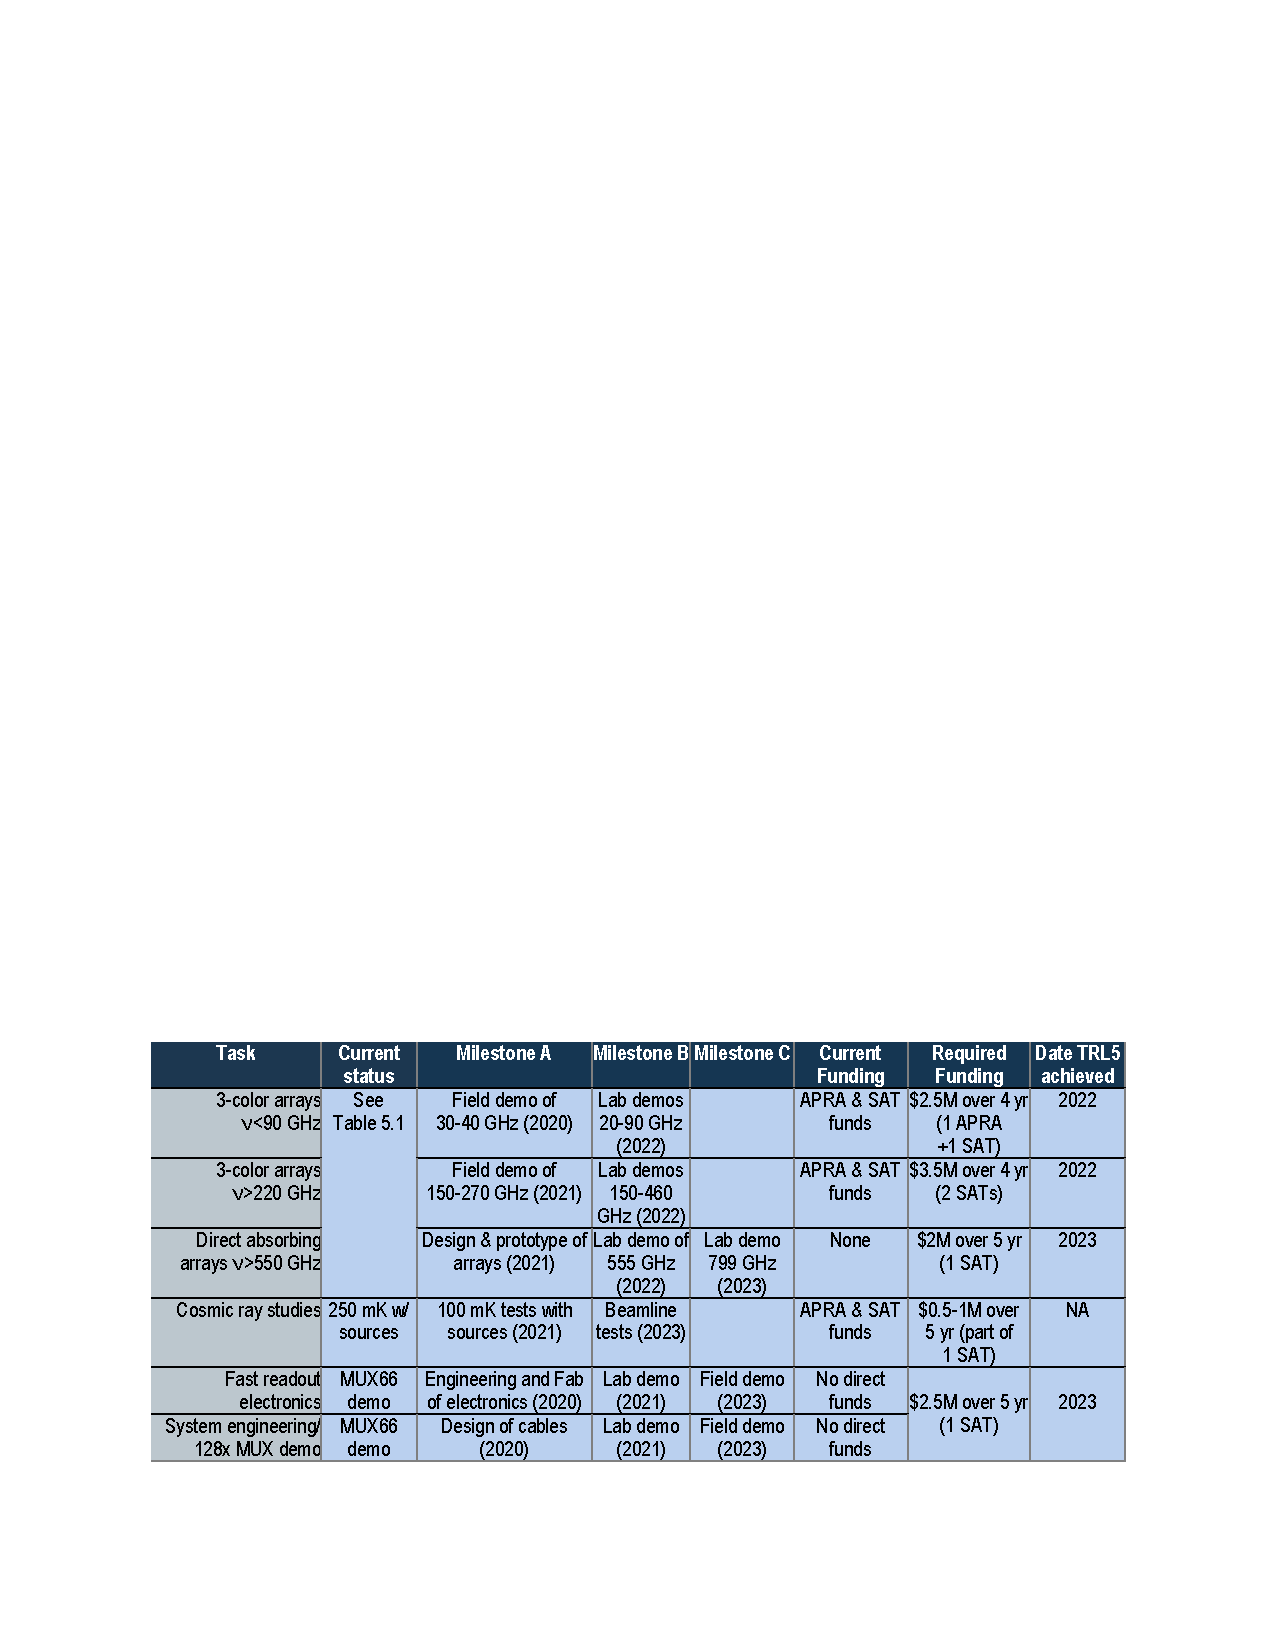
\includegraphics{tables/tab_technologies.pdf}
% \begingroup
% \setlength{\tabcolsep}{0.5em} 
% \renewcommand{\arraystretch}{1.3} % Default value: 1
% \footnotesize\rmfamily
% \begin{tabular}{lp{1.0in}p{0.75in}p{0.75in}p{0.6in}p{0.6in}p{0.5in}p{0.5in}p{0.4in}}
% \hline\noalign{\vskip3pt}
% &\bfseries Task & \bfseries Current status & \bfseries Milestone A &\bfseries Milestone B &\bfseries Milestone C &\bfseries Current funding &\bfseries Required Funding & \bfseries TRL5 achieved \\ 
% \noalign{\vskip3pt}\hline\noalign{\vskip3pt}
% 1a.&\parbox[t]{\columnwidth}{Three-color arrays\\$\nu<90$\,GHz} & 2-color lab demos $\nu > 30$\,GHz & Field demo of 30--40\,GHz (2020) & Lab demos 20--90 GHz (2022) & -- & APRA \& SAT funds & \$2.5M over 4\,yr (1 APRA + 1 SAT) & 2022 \\ %\hline
% 1b&\parbox[t]{\columnwidth}{Three-color arrays\\$\nu > 220$\,GHz} & 2-color lab demos $\nu < 300$\,GHz& Field demo of 150--270\,GHz (2021) &  & -- & APRA \& SAT funds & \$3.5M over 4\,yr (2 SATs) & 2022 \\ %\hline
% 2.&\parbox[t]{\columnwidth}{Direct absorbing\\arrays $\nu > 50$\,GHz}& 0.1--5\,THz unpolarized&Design \& prototype of arrays (2021)&Lab demo of 555\,GHz (2022)& Lab demo 799\,GHz (2023) & None & \$2M over 5\,yr (1 SAT) & 2023 \\ %\hline
% 3.&\parbox[t]{\columnwidth}{Cosmic ray studies}& 250\,mK w/ sources&100\,mK tests with sources (2021)&Beamline tests (2023)& -- & APRA \& SAT funds & \$0.5--1M over 5\,yr (part of 1 SAT) & NA \\ %\hline
% 4a.&\parbox[t]{\columnwidth}{Fast readout\\electronics}& MUX66 demo&Engineering and Fab of electronics (2020)&Lab demo (2021)&Field demo (2023)& No direct funds & \multirow{2}{*}{\parbox[c]{\columnwidth}{\vskip 2.5em\$4M over\\ 5\,yr (1 SAT)}} & \multirow{2}{*}{\parbox[c]{\columnwidth}{\vskip 3em 2023}} \\ %\cline{1-7}
% 4b.&\parbox[t]{\columnwidth}{System engineering;\\ 128x MUX demo} & MUX66 demo &Design of cables (2020)&Lab demo (2021)& Field demo (2023) & No direct funds &  &  \\ %\hline
% \noalign{\vskip3pt}\hline
% \end{tabular}
% \endgroup
% \end{center}
% \end{table}
